\documentclass{article}
\usepackage{csquotes}
\usepackage[utf8x]{inputenc}
\usepackage[T1,T2A]{fontenc}
\usepackage{fvextra}
\fvset{commandchars=\\\{\}, mathescape=true}
\usepackage{xcolor}
\usepackage{amssymb}       % define \Sha
\usepackage{listings}
\usepackage{listingsutf8}
\usepackage[spanish]{babel}
\usepackage{graphicx}
\usepackage[style=ieee]{biblatex} % Establecer el estilo de las referencias como IEEE
\usepackage{hyperref}
\usepackage{titletoc}
\usepackage{adjustbox}

\definecolor{bg}{rgb}{0.95,0.95,0.95}
\definecolor{gray}{rgb}{0.5,0.5,0.5}
\definecolor{purple}{rgb}{0.58,0,0.82}
\definecolor{bluekeyword}{rgb}{0.26,0.44,0.76}
\definecolor{lightorange}{rgb}{0.8,0.5,0.2}
\definecolor{darkgreen}{rgb}{0.0,0.5,0.0}

\lstdefinestyle{mypython}{
    inputencoding=utf8,           % Indica a listings que use UTF-8
    extendedchars=true,           % Permite caracteres extendidos
    mathescape=true,              % Habilita modo matemático dentro de literales
    language=Python,
    backgroundcolor=\color{bg},
    basicstyle=\ttfamily\footnotesize,
    keywordstyle=\color{bluekeyword}\bfseries,
    commentstyle=\color{gray}\itshape,
    stringstyle=\color{lightorange},
    numberstyle=\tiny\color{gray},
    identifierstyle=\color{black},
    showstringspaces=false,
    numbers=left,
    numbersep=10pt,
    frame=single,
    breaklines=true,
    tabsize=4,
    captionpos=b,
    escapeinside={(*@}{@*)},
    literate=
     {á}{{\'a}}1 {é}{{\'e}}1 {í}{{\'i}}1 {ó}{{\'o}}1 {ú}{{\'u}}1
     {Á}{{\'A}}1 {É}{{\'E}}1 {Í}{{\'I}}1 {Ó}{{\'O}}1 {Ú}{{\'U}}1
     {ñ}{{\~n}}1 {Ñ}{{\~N}}1 {π}{{$\pi$}}1  {Ш}{{\fontencoding{T2A}\selectfont\char"DB}}1
     {¡}{{\textexclamdown}}1 {¿}{{\textquestiondown}}1
}


\hypersetup{
    colorlinks=true,
    linkcolor=blue, % Color del texto del enlace
    urlcolor=blue % Color del enlace
}

\usepackage{longtable} % Agrega el paquete longtable

\definecolor{mygreen}{RGB}{0,128,0}

\usepackage{array} % Para personalizar la tabla
\usepackage{booktabs} % Para líneas horizontales de mejor calidad
\usepackage{graphicx} % Paquete para incluir imágenes
\usepackage{float}
\usepackage[section]{placeins}

% Definir márgenes
\usepackage[margin=1in]{geometry}

\renewcommand{\contentsname}{\textcolor{mygreen}{Tabla de Contenidos}}

\begin{document}

\begin{titlepage}
  \centering
  % Logo de la Universidad
  
\includegraphics[width=0.48\textwidth]{logo_universidad.png}
  \par\vspace{2cm}

  % Nombre de la Universidad y detalles del curso
  {\Large \textbf{Universidad Nacional de Colombia} \par}
  \vspace{0.5cm}
  {\large Ingeniería de Sistemas y Computación \par}
  {\large 2025966 Lenguajes de Programación (02)\par}
  \vspace{3cm}

  % Detalles del laboratorio y actividad
  {\large \textbf{Taller 1} \par}
  {\large Analizador Léxico\par}
  \vspace{3cm}

  % Lista de integrantes
  {\large \textbf{Integrantes:} \par}
  \vspace{0.5cm}
  \begin{tabular}{ll}
    Javier Andrés Tarazona Jiménez & jtarazonaj@unal.edu.co \\
    David Felipe Marin Rosas       & dmarinro@unal.edu.co   \\
    Juan Sebastian Muñoz Lemus     & jumunozle@unal.edu.co          \\
  \end{tabular}
  \par\vspace{3cm}

  % Fecha
  {\large Junio 24 de 2025 \par}
\end{titlepage}

\tableofcontents % Inserta la tabla de contenidos

\newpage % Salto de página para separar la tabla de contenidos del contenido del documento

% Contenido del artículo----------------------------------------------------------

%---------------------------------------------------------------------------------
% Intro --------------------------------------------------------------------------
%---------------------------------------------------------------------------------

\section{Introducción}\label{sec:intr}

En el desarrollo de lenguajes de programación, el diseño e implementación de 
analizadores léxicos constituye uno de los pilares fundamentales para garantizar 
que la interpretación y procesamiento del código fuente sea precisa, robusta 
y escalable. En este taller, se propuso no solo abordar la construcción de un 
analizador léxico para un lenguaje de dominio específico orientado a pruebas 
estadísticas tipo Friedman y análisis de rachas, sino también entender a profundidad 
los retos prácticos que esto implica desde la perspectiva del diseño modular, 
el uso de expresiones regulares y la integración de herramientas modernas en 
Python como PLY. Mmás allá de la simple clasificación de 
cadenas, se explora cómo el reconocimiento léxico bien estructurado sienta las 
bases para sistemas de compilación eficientes, confiables y alineados con 
los conceptos de programación imperativa y la abstracción de estructuras de 
datos. Este trabajo busca que cada componente del lexer utilizado contribuya 
de manera significativa tanto a la formación profesional como al 
avance en la construcción de soluciones computacionales adaptadas a 
necesidades específicas en estadística y análisis de datos experimentales.

%---------------------------------------------------------------------------------
% Marco Teórico ------------------------------------------------------------------
%---------------------------------------------------------------------------------

\section{Marco Teórico}\label{sec:marc}


\subsection{Contextualización del problema}

En el ámbito de la estadística matemática, el análisis no paramétrico juega un papel fundamental cuando no se cumplen los supuestos clásicos de normalidad o cuando los datos tienen una naturaleza ordinal. En este contexto, las \textbf{pruebas de Friedman} se utilizan ampliamente para evaluar diferencias entre tratamientos o condiciones en experimentos de medidas repetidas. La prueba de Friedman, propuesta por Milton Friedman en 1937, es una alternativa no paramétrica al análisis de varianza de medidas repetidas (ANOVA de una vía con medidas repetidas), y se basa en el análisis de los \emph{rangos} en lugar de los valores originales.

Un concepto complementario a estas pruebas es la \textbf{teoría de rachas}, que consiste en analizar secuencias de datos categóricos o binarios con el fin de identificar patrones de aleatoriedad. Una \emph{racha} es una secuencia de elementos iguales consecutivos en un conjunto de datos. Esta teoría es clave en pruebas de hipótesis sobre la independencia o aleatoriedad de observaciones sucesivas, y tiene aplicaciones en diversas áreas, como pruebas estadísticas, control de calidad, genética y ciencias sociales.

Dado el uso intensivo de estos métodos en investigación y análisis de datos, surge la necesidad de contar con herramientas computacionales que faciliten su aplicación, integración y extensión. Para ello, el desarrollo de un \textbf{lenguaje de programación de propósito específico} (DSL, por sus siglas en inglés) orientado a estas pruebas representa una solución efectiva. Este lenguaje debe permitir expresar de manera clara, concisa y semánticamente válida los procedimientos relacionados con las pruebas de Friedman y el análisis de rachas, integrando estructuras de programación tradicionales como variables, arreglos, matrices, ciclos y condicionales.


%---------------------------------------------------------------------------------
% Descripción y Justificación del Problema a Resolver ----------------------------
%---------------------------------------------------------------------------------

\section{Descripción y Justificación del Problema a Resolver}\label{sec:descr}

\subsection{Descripcion del problema}

El problema a resolver consiste en el diseño y construcción de la primera etapa de un \textbf{lenguaje de programación de propósito específico}, enfocado en facilitar la implementación de pruebas estadísticas como la de Friedman y el análisis de rachas. Este lenguaje deberá permitir a los usuarios (principalmente profesionales en estadística) desarrollar programas que manipulen datos experimentales, realicen ordenamientos por rangos, detecten rachas y apliquen criterios de hipótesis sobre la aleatoriedad de los datos.

El lenguaje será construido bajo el \textbf{paradigma imperativo}, lo que implica que el flujo de control de los programas estará compuesto por \textbf{secuencias de instrucciones, estructuras de selección (\texttt{if}, \texttt{switch}), iteración (\texttt{for}, \texttt{while})} y el uso de \textbf{tipos de datos abstractos (TDA)}. Además, debe incorporar capacidades para definir y trabajar con \textbf{variables, arreglos unidimensionales y matrices}, elementos comunes en los procesos de manipulación de datos experimentales.

En esta primera fase, se enfoca específicamente en el \textbf{análisis léxico} del lenguaje, es decir, la definición del vocabulario que podrá ser reconocido por el compilador o intérprete, la clasificación de los elementos léxicos (\emph{tokens}), y su implementación práctica mediante una herramienta de análisis léxico como \textbf{FLEX} (para C), \textbf{JFLEX} (para Java) o \textbf{lex.py} (para Python).

\subsection{Justificacion del problema}

La justificación del proyecto radica en la necesidad de herramientas especializadas para el análisis estadístico avanzado, que actualmente se realiza mediante lenguajes de propósito general como R, Python o MATLAB, los cuales requieren de una curva de aprendizaje considerable y conocimientos de programación más generales. Un lenguaje específico para pruebas de Friedman y análisis de rachas permitirá:

\begin{itemize}
  \item \textbf{Reducir la complejidad} de la codificación de estas pruebas.
  \item \textbf{Establecer una sintaxis especializada} que se alinee con los conceptos estadísticos que utilizan los profesionales del área.
  \item \textbf{Evitar errores semánticos comunes}, al estar restringido a un dominio de aplicación concreto.
  \item \textbf{Agilizar el análisis y la validación de hipótesis estadísticas} sin necesidad de implementar desde cero las pruebas cada vez.
\end{itemize}

Además, desde el punto de vista académico, el desarrollo de este lenguaje contribuye a la formación integral en diseño de lenguajes, compiladores y en la aplicación del paradigma imperativo mediante el diseño modular de analizadores léxicos.


\subsection{Objetivo Principal}

\begin{quote}
Diseñar e implementar el analizador léxico de un lenguaje de programación de propósito específico orientado a pruebas estadísticas de dos vías de clasificación, basadas en la teoría de rachas y pruebas tipo Friedman, utilizando el paradigma de programación imperativo y estructuras abstractas de datos.
\end{quote}

Este objetivo general se descompone en las siguientes metas específicas:

\begin{itemize}
  \item Proponer prototipos de programas que ejemplifiquen cómo se utilizaría el lenguaje para expresar problemas de análisis estadístico.
  \item Definir el vocabulario del lenguaje y las categorías léxicas necesarias.
  \item Formalizar los patrones léxicos mediante expresiones regulares.
  \item Implementar el analizador léxico en una herramienta adecuada (FLEX, JFLEX o lex.py).
\end{itemize}
%---------------------------------------------------------------------------------
% Diseño de la solución ---------------------------------------------------------
%---------------------------------------------------------------------------------

\section{Diseño de la solución}\label{sec:dis}


La solución se organiza en un pipeline modular de seis capas que separa 
las responsabilidades, el diagrama se puede ver en la imagen \ref{fig:pipelineLexico}.
El \emph{Lector de Archivo} se encarga de la lectura 
del archivo fuente completo, enviado como un .txt. Este es el
un código del lenguaje al que se le quiere pasar el analizador léxico.

A continuación, la \emph{Capa de Preprocesamiento} filtra espacios y tabulaciones 
(o bien lleva la cuenta de líneas cuando se requiera).

La \emph{Capa de Construcción del Lexer} utiliza \texttt{PLY} con banderas 
\texttt{re.VERBOSE} compilando en una sola estructura los patrones de expresión 
regular. Esto facilita el análisis para expresiones de regex
complejas, como las que se usan al combinar
lad funciones de python (fprints) con el propio regex.

El \emph{Motor de Tokenización} recorre la entrada con las reglas definidas y, 
finalmente, en la \emph{Capa de Salida}, se envían los tokens etiquetados 
con su tipo, valor, línea y posición en un archivo de salida, 
listo para las fases posteriores del compilador.

\begin{figure}[ht]
  \centering
  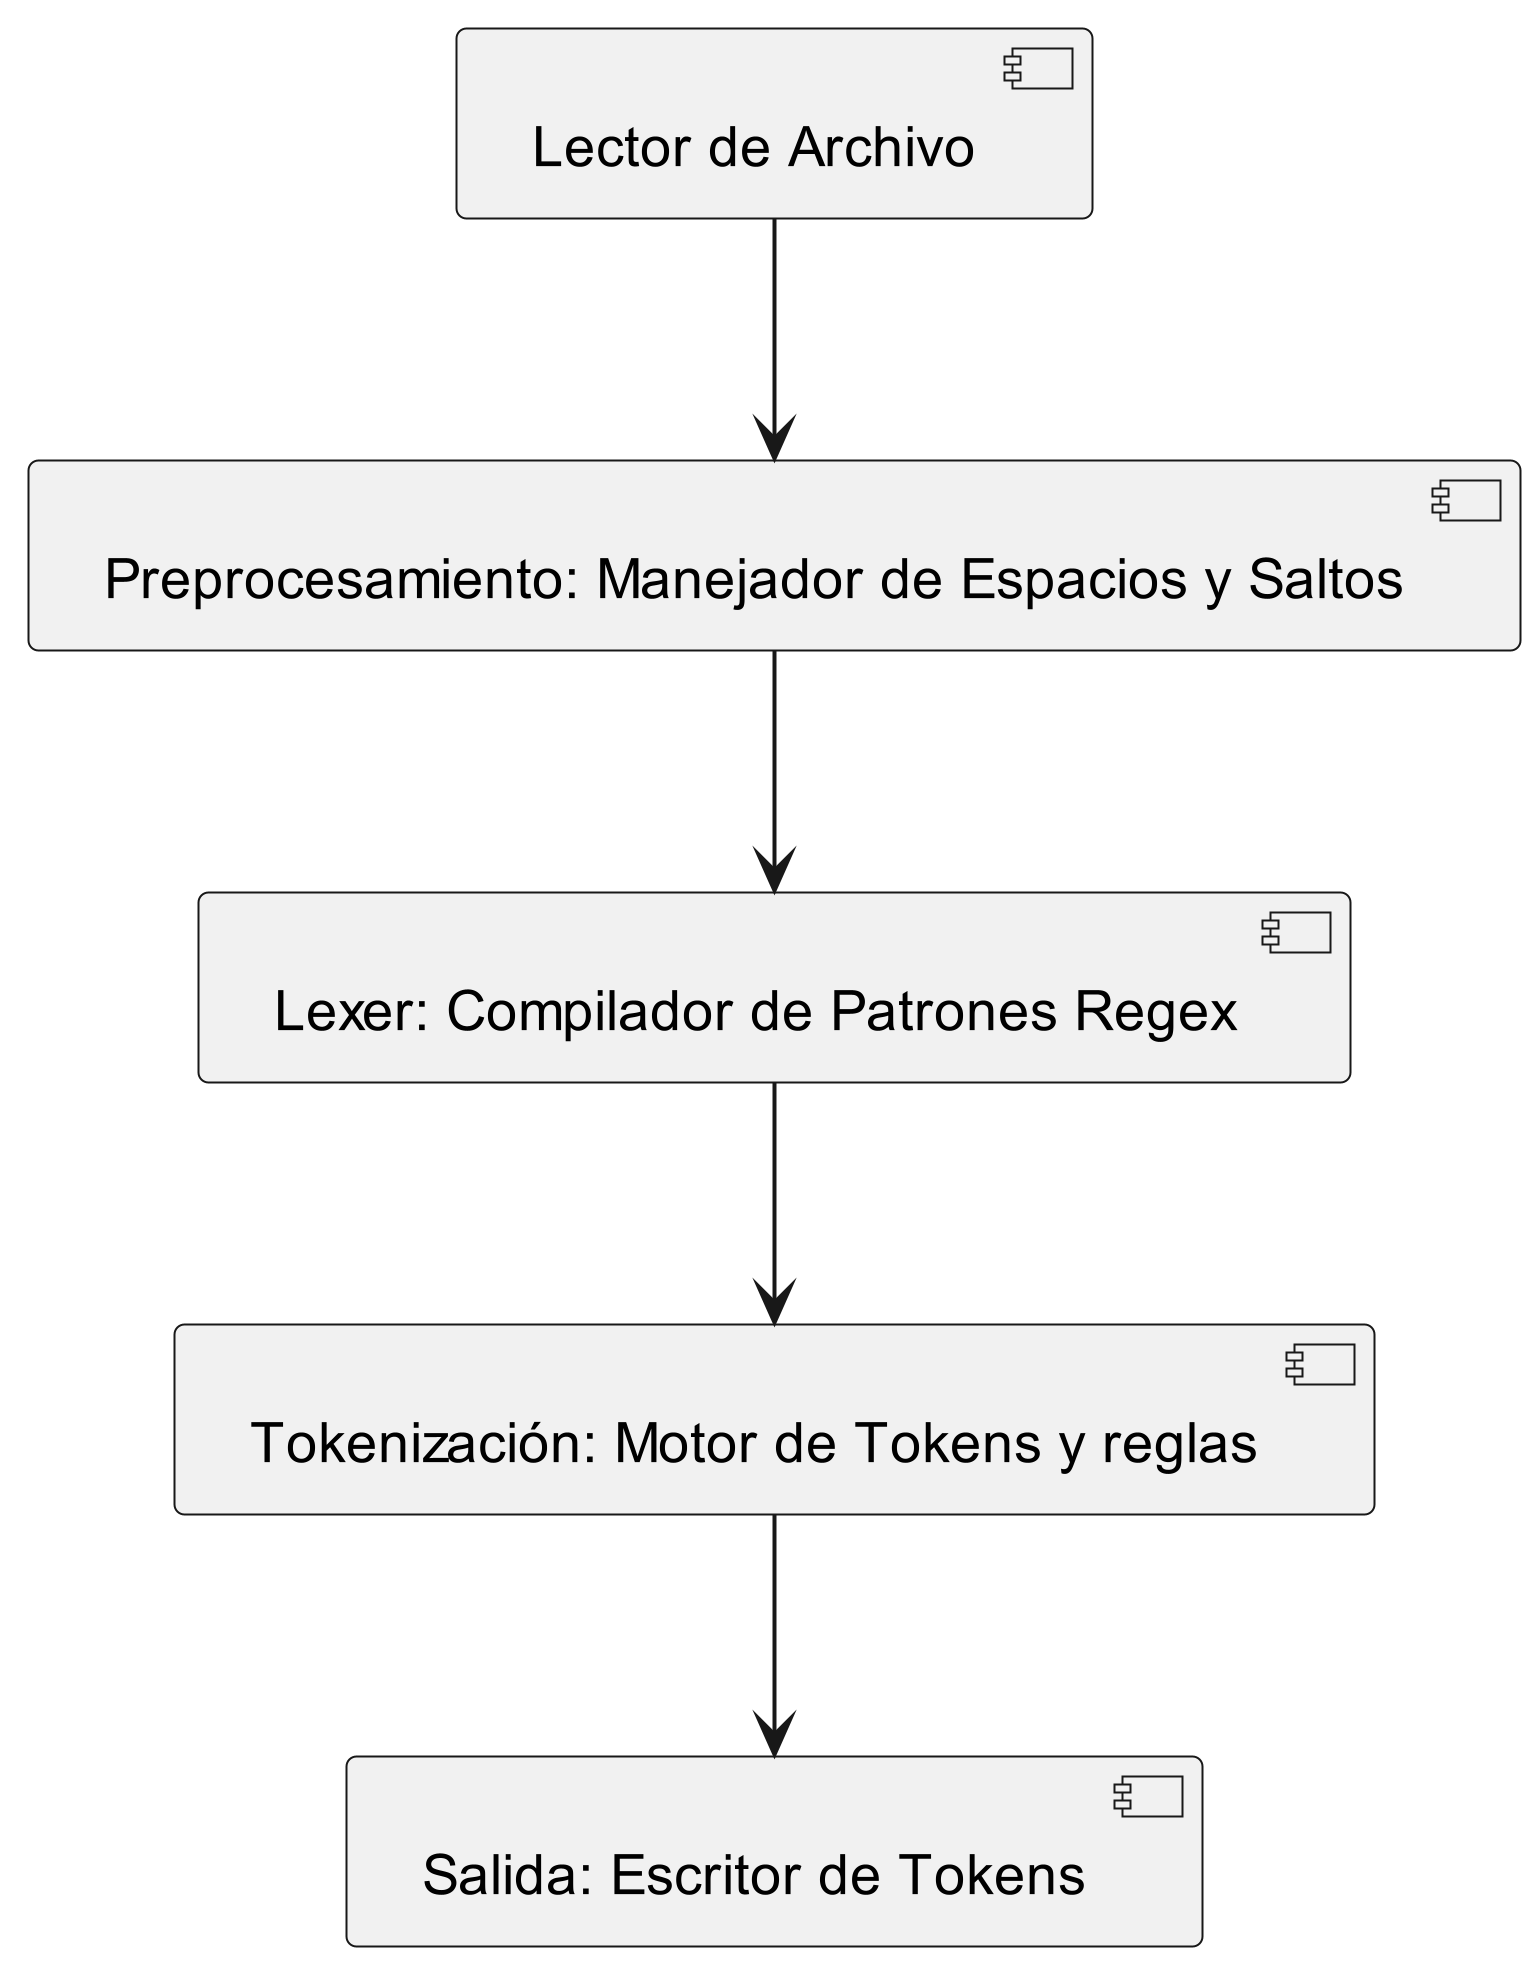
\includegraphics[width=0.7\textwidth]{Flujo.png}
  \caption{Pipeline modular del analizador léxico por capas}
  \label{fig:pipelineLexico}
\end{figure}

\vspace{1em}

En la imagen \ref{fig:MotorTokens1} y \ref{fig:MotorTokens2}
 se pueden ver las categorías léxicas que se implementaron como
reglas del motor de tokens.

\begin{figure}[ht]
  \centering
  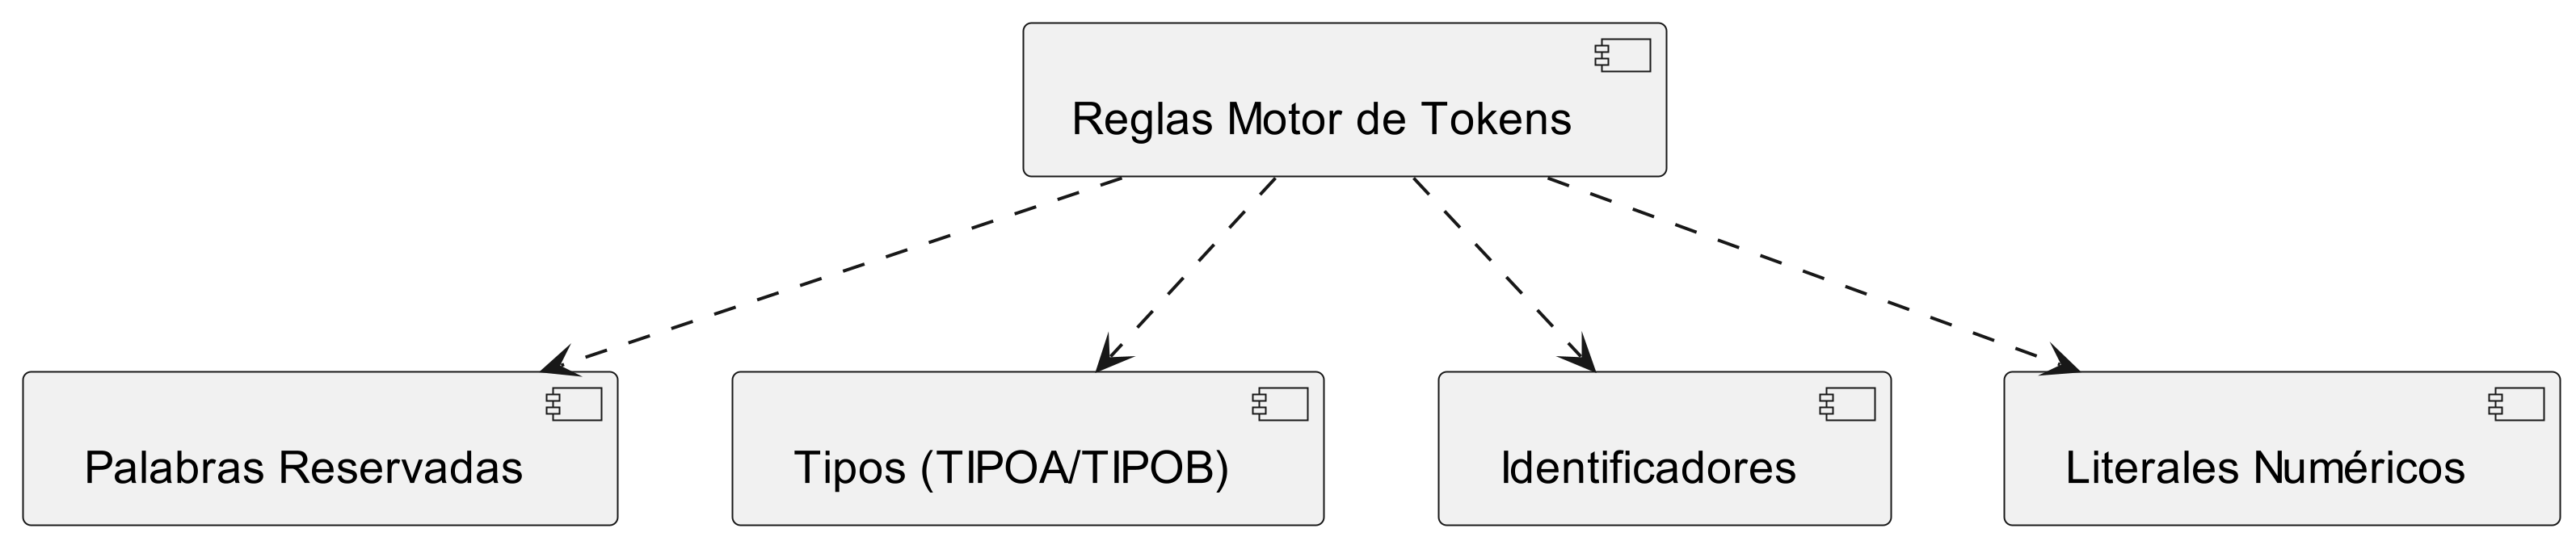
\includegraphics[width=1\textwidth]{MotorTokens1.png}
  \caption{Motor de Tokens Parte 1}
  \label{fig:MotorTokens1}
\end{figure}

\begin{figure}[ht]
  \centering
  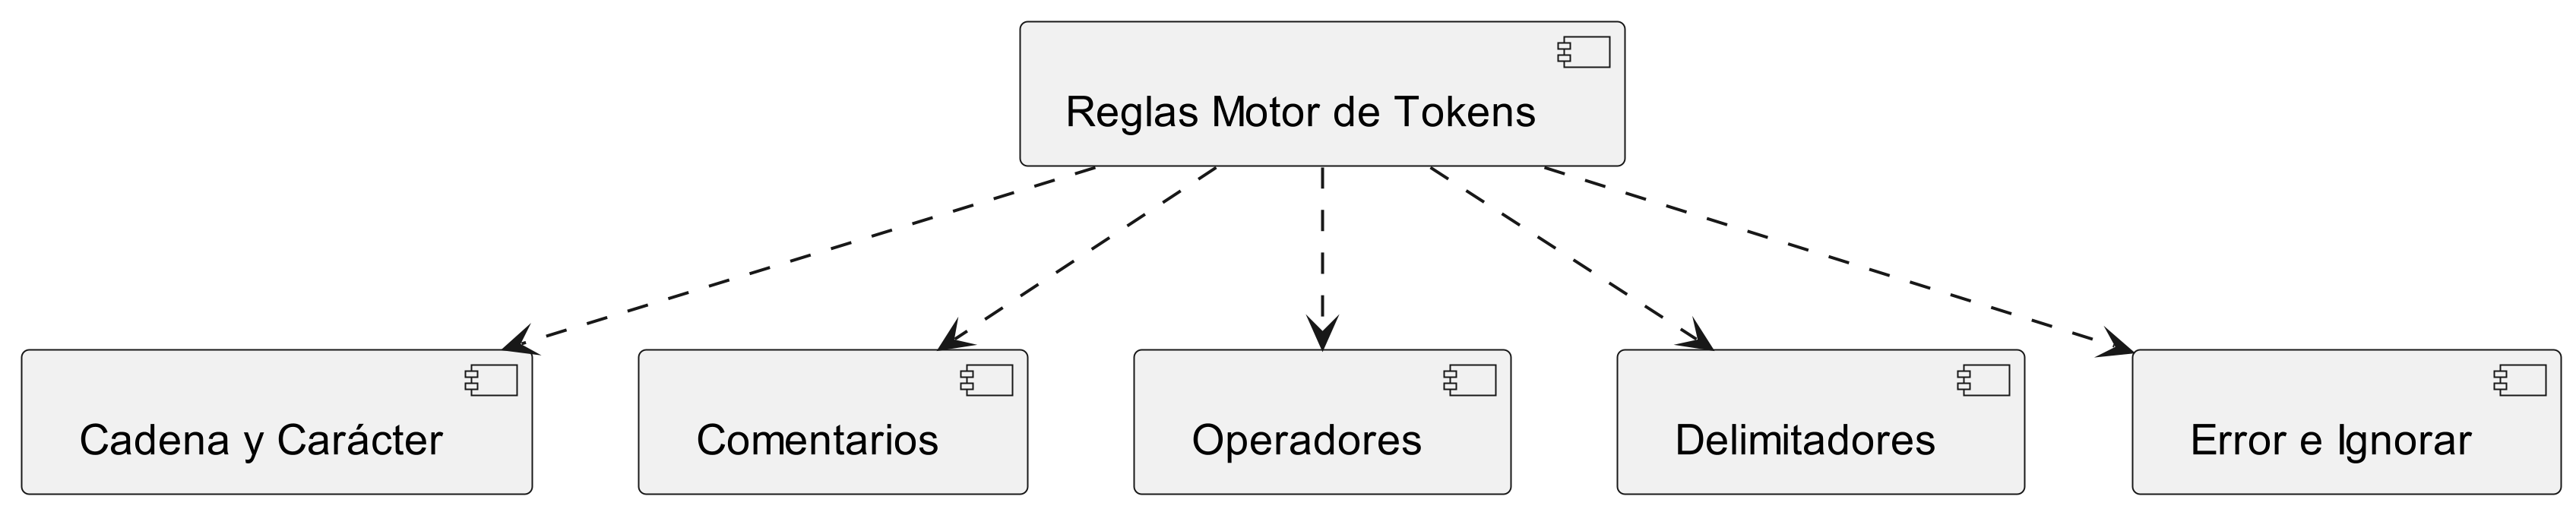
\includegraphics[width=1\textwidth]{MotorTokens2.png}
  \caption{Motor de Tokens Parte 2}
  \label{fig:MotorTokens2}
\end{figure}


\noindent Cada categoría de token se implementa de forma aislada para evitar 
solapamientos:
\begin{itemize}
  \item Las palabras reservadas, \texttt{TIPOA} y \texttt{TIPOB}
      se manejan mediante un único \texttt{t\_ID} que consulta un diccionario 
      \texttt{reserved}, garantizando prioridad a los tipos compuestos 
      (\texttt{Conjunto<T>}, \texttt{MatrizRachas<T>}\dots) antes de clasificar 
      como identificador.
  \item Los literales numéricos aplican precedencia 
      (complejo \(\rightarrow\) real \(\rightarrow\) entero) mediante tres reglas 
        con docstrings, asegurando que expresiones 
        como \texttt{1+2j}, \texttt{3.14e-2} y \texttt{42} se reconozcan correctamente.
  \item Para cadenas y caracteres, se definen patrones robustos 
    que admiten escapes y placeholders (incluyendo soporte para la ñ/Ñ 
    en identificadores), y para comentarios, una regla de función 
    \texttt{t\_COMMENT} captura \texttt{//…} y \texttt{/*…*/} antes de que 
    intervengan los operadores. Se añade que se ponen al inicio para que no 
    se solapen con otras categorías léxicas.
  \item Finalmente, las expresiones de operadores y delimitadores se 
    definen como literales agrupados y ordenados por longitud, 
    evitando ambigüedades gracias al orden de declaración. Por
    ejemplo entre \texttt{!=} y \texttt{!}.
\end{itemize}


%---------------------------------------------------------------------------------
% Código Fuente ---------------------------------------------------------
%---------------------------------------------------------------------------------

\section{Código Fuente}\label{sec:cod}

El código fuente completo de este modelo se encuentra adjunto como 
(taller1.zip)
y disponible en el repositorio GitHub del proyecto:

\begin{center}
\url{https://github.com/JavierTarazona06/LP02_Tareas/tree/main/taller1/code}
\end{center}

%---------------------------------------------------------------------------------
% Manual Usuario ---------------------------------------------------------
%---------------------------------------------------------------------------------

\section{Manual Usuario}\label{sec:man_u}

El primer paso es descargar el archivo \texttt{taller1.zip}.

El repositorio contiene:
\begin{itemize}
  \item \textbf{Código principal}
  \begin{description}
    \item[\texttt{a\_lexico.py}] Código principal del analizador léxico: 
      define la lista de tokens, patrones (regex) y funciones \texttt{t\_…} que definen patrones
      para cada categoría, y construye el lexer con PLY.
  \end{description}

  \item \textbf{Otros}
  \begin{description}
    \item[\texttt{InstallationGuide.md}] Guía paso a paso (Markdown) para crear y 
      activar el entorno virtual y luego instalar las dependencias necesarias con 
      \texttt{pip install -r requirements.txt}.
    \item[\texttt{requirements.txt}] Lista de dependencias del proyecto 
      (principalmente la versión de \texttt{ply} necesaria para ejecutar el analizador).
  \end{description}

  \item \textbf{Testing}
  \begin{description}
    \item[\texttt{tests/prototype1.txt}] Primer caso de prueba: un 
      fragmento de código del lenguaje fuente (teoría de rachas) propuesto para verificar el lexer.
    \item[\texttt{tests/prototype1\_lex.txt}] Salida esperada del lexer al 
        procesar \texttt{prototype1.txt}, listando línea:posición, tipo de token y lexema.
    \item[\texttt{tests/prototype2.txt}] Segundo caso de prueba: ejemplo con estructuras de 
        datos (matrices, arreglos) y tipado flotante del lenguaje propuesto.
    \item[\texttt{tests/prototype2\_lex.txt}] Tokens generados por el lexer para el contenido 
        de \texttt{prototype2.txt}.
    \item[\texttt{tests/prototype3.txt}] Tercer caso de prueba: implementación 
        del algoritmo de Euclides en el lenguaje propuesto
    \item[\texttt{tests/prototype3\_lex.txt}] Salida de tokens correspondiente al 
        archivo \texttt{prototype3.txt}.
    \item [\texttt{tests/escenarioPrueba...}] Archivos relacionados a los escenarios de prueba.
  \end{description}
\end{itemize}


Una vez descargado, descomprímalo y acceda a la carpeta. Dentro de ella, cree un 
entorno virtual utilizando Python 3.10. o superior. Para ello, ejecute el siguiente 
comando en 
la terminal o línea de comandos:

\begin{itemize}
  \item En Windows:
        \begin{verbatim}
    python3.12 -m venv nombre_del_entorno
  \end{verbatim}
  \item En macOS o Linux:
        \begin{verbatim}
    python3.12 -m venv nombre_del_entorno
  \end{verbatim}
\end{itemize}

Donde \texttt{nombre\_del\_entorno} es el nombre que desea asignar a su entorno virtual.
A continuación, active el entorno virtual:

\begin{itemize}
  \item En Windows:
        \begin{verbatim}
    .\nombre_del_entorno\Scripts\activate
  \end{verbatim}
  \item En macOS o Linux:
        \begin{verbatim}
    source nombre_del_entorno/bin/activate
  \end{verbatim}
\end{itemize}

Asegúrese de tener el entorno virtual activado. 
A continuación, descargue las dependencias necesarias 
(en este caso, únicamente \texttt{PLY} para gestionar \texttt{Lex}):

\begin{verbatim}
    pip install -r requirements.txt
\end{verbatim}

Una vez activo y el entorno instalado, puede ejecutar el archivo 
principal con el siguiente comando:

\begin{center}
  \begin{adjustbox}{minipage=\linewidth, center}
  \begin{verbatim}
    python a_lexico.py
  \end{verbatim}
  \end{adjustbox}
\end{center}

\begin{enumerate}
  \item Al iniciar el analizador, la terminal mostrará el prompt:
    \begin{verbatim}
      term>
    \end{verbatim}
    y permanecerá a la espera de que se introduzca la ruta completa (\texttt{path}): 
    la dirección, el nombre y la extensión del archivo fuente que contiene 
    el código en el lenguaje propuesto.
    \\
    \textbf{Ejemplo:}
    \begin{verbatim}
      term> C:\proyectos\mi_codigo.txt
    \end{verbatim}

    Cabe resaltar que no toca especificar el path, si el archivo
    se encuentra en current directory.

  \item Una vez recibida la ruta, el analizador léxico leerá y procesará ese archivo.

  \item A continuación, generará un archivo de salida en el \emph{mismo directorio},
    con el \emph{mismo nombre} que el original y el sufijo \_\texttt{lex.txt}.
    \\
    \textbf{Si el archivo de entrada es}
    \begin{verbatim}
        C:\proyectos\mi_codigo.txt
    \end{verbatim}
    \textbf{el analizador creará}
    \begin{verbatim}
      C:\proyectos\mi_codigo_lex.txt
    \end{verbatim}

  \item El contenido de \texttt{mi\_codigo\_lex.txt} 
    será el análisis léxico completo. Cada línea incluirá:
    \begin{itemize}
      \item \textbf{Posición}: por ejemplo, línea:columna o un offset numérico.
      \item \textbf{Tipo de token}: por ejemplo, \texttt{ID}, \texttt{ENTERO}, \texttt{PALABCLAVE}.
      \item \textbf{Lexema}: el texto exacto reconocido.
    \end{itemize}
    \textbf{Ejemplo de línea de salida:}
    \begin{verbatim}
      3:15    ID        contador
      3:23    OPARIT    =
      3:25    ENTERO    42
    \end{verbatim}
\end{enumerate}

%---------------------------------------------------------------------------------
% Manual Técnico ---------------------------------------------------------
%---------------------------------------------------------------------------------

\section{Manual Técnico}\label{sec:man_t}

\subsection{Resumen}

Esta sección describe la construcción de un analizador léxico usando la biblioteca \texttt{ply.lex} en Python. El objetivo es reconocer estructuras léxicas propias de un lenguaje de programación personalizado, incluyendo identificadores, palabras clave, operadores, tipos, literales y delimitadores.

\subsection{Estructura General}

A continuación se detalla la estructura general del código:

\begin{itemize}
  \item El código usa la biblioteca \texttt{ply.lex} para definir un lexer que procesa un texto fuente y genera tokens. Cada token es una unidad léxica que representa una categoría específica del lenguaje.
  \item El codigo cuenta con dos partes principales, en la primera se definen los tokens (\texttt{tokens}), las palabras reservadas (\texttt{reserved}) y las funciones o expresiones regulares (aquellas que empiezan por \texttt{t\_}) que definen la estructura del lenguajes, en la segunda parte, se define la función \texttt{\_\_main\_\_} en la cual se pide la dirección de un archivo que contiene el texto a ser procesado, después de leer el contenido de este archivo, se procesa y se guarda en un archivo con el mismo nombre pero sin la extensión y con la terminación \texttt{\_tokens.txt}.
  \item Al principio del codigo se declara una lista vacia de tokens que luego se va llenando con las categorías que el analizador puede reconocer, aquí también se define la variable \texttt{reserved} usada para definir las palabras clave que pertenecen a una categoria. El código se organiza en varias secciones que definen las categorías y subcategorías dentro de estas (tokens, palabras reservadas, tipos de datos, cadenas, identificadores, literales numéricos, comentarios y operadores), en cada una de estas secciones se van agregando las cadenas de caracteres que representan los tipos de tokens correspondientes a la categoría (a la lista \texttt{tokens}) y a sus subcategorías correspondientes (dentro del diccionario \texttt{reserved}), se crean las expresiones regulares o los mecanismos de reconocimiento para cada categoria bajo las funciones \texttt{t\_<nombre\_categoria>} y bajo su atributo \texttt{\_\_doc\_\_}.
\end{itemize}

\subsection{Categorías definidas:}

\subsubsection{PALABCLAVE}

Esta sección define las palabras clave del lenguaje. Estas palabras tienen un significado especial dentro de la gramática y no pueden usarse como identificadores por el usuario. Se agrupan en una lista y se registran en un diccionario reservado para ser reconocidas durante el análisis léxico.

\begin{lstlisting}[style=mypython]
  tokens.append('PALABCLAVE')

  palabras_reservadas = [
      'Func','Principal','imprimir','Vacio','Retornar','Global',
      'Romper','Continuar','Pasar','Sino',
      'Si','Entonces','Para','Mientras','Lanzar','Intentar',
      'Excepto'
  ]
  reserved = { w: 'PALABCLAVE' for w in palabras_reservadas }
  \end{lstlisting}

\subsubsection{TIPO}

Define los tipos de datos del lenguaje. Se separan en tipos atómicos (como \texttt{Entero} o \texttt{Bool}) y tipos estructurados (como \texttt{Matriz} o \texttt{Diccionario}). Cada uno se mapea a su token correspondiente (\texttt{TIPOA} o \texttt{TIPOB}) para su correcta clasificación.

\begin{lstlisting}[style=mypython]
tokens += ['TIPOA', 'TIPOB']

tiposa = ['Bool','Entero','Flotante','Cadena','Caracter']
reserved.update({ w: 'TIPOA' for w in tiposa})

tiposb = ['Conjunto','Arreglo','Matriz','MatrizRachas','Multicotomizacion','M2VClasificacion','Diccionario']
reserved.update({ w: 'TIPOB' for w in tiposb })
\end{lstlisting}

\subsubsection{Caracter y Cadenas}

Esta sección define cómo se reconocen los caracteres y cadenas. Los caracteres están definidos por comillas simples y las cadenas pueden ser simples o contener expresiones interpoladas (estilo \texttt{f-strings}).

\begin{lstlisting}[style=mypython]
tokens += ['CARACTER', 'CADENA']

t_CARACTER = r"'(?:\\.|[^\\'])'"

CADENA_S = r'"(?:\\.|[^"\\])*"'
CADENA_F = (
    r'"(?:'
    r'\\.'
    r'|[^"\\{]'
    r'|\{[A-Za-z_][A-Za-z0-9_]*\}'
    r')*"'
)
CADENA_PATTERN = rf'(?:{CADENA_S}|{CADENA_F})'

def t_CADENA(t):
    return t
t_CADENA.__doc__ = CADENA_PATTERN
\end{lstlisting}

\subsubsection{ID}

Los identificadores se reconocen como cualquier secuencia válida que comience con una letra o guión bajo, seguida de letras, números o guión bajo. Si el valor coincide con una palabra reservada, se clasifica como tal, si no, como \texttt{ID}.

\begin{lstlisting}[style=mypython]
tokens += ['ID', 'BOOL']

reserved.update({ b: 'BOOL' for b in ['Verdadero','Falso'] })

def t_ID(t):
    r'[A-Za-z_][A-Za-z0-9_]*'
    t.type = reserved.get(t.value, 'ID')
    return t
\end{lstlisting}

\subsubsection{LITERAL}

Reconoce valores literales numéricos. Incluye enteros (\texttt{ENTERO}), números reales con punto decimal (\texttt{REAL}) y números complejos (\texttt{COMPLEJO}). Cada tipo convierte su lexema al tipo de dato adecuado.

\begin{lstlisting}[style=mypython]
tokens += ['ENTERO','REAL','COMPLEJO']

DIGITO = r'[0-9]'
NATURAL = rf'(?:[1-9]{DIGITO}*|0)'
ENTERO_PATTERN = rf'(?:-?{NATURAL})'
REAL_U = rf'(?:{NATURAL}?\.{NATURAL})(?:[eE][+-]?{NATURAL})?'
REAL_PATTERN = rf'(?:-?{REAL_U})'
COMPLEJO_PATTERN = rf'(?:{REAL_PATTERN}[+-]{REAL_U}[jJ]|{REAL_PATTERN}[jJ])'

def t_COMPLEJO(t):
    t.value = complex(t.value.replace('J','j'))
    return t
t_COMPLEJO.__doc__ = COMPLEJO_PATTERN

def t_REAL(t):
    t.value = float(t.value)
    return t
t_REAL.__doc__ = REAL_PATTERN

def t_ENTERO(t):
    t.value = int(t.value)
    return t
t_ENTERO.__doc__ = ENTERO_PATTERN
\end{lstlisting}

\subsubsection{COMMENT}
Define los comentarios del lenguaje. Se reconocen tanto los de línea (\texttt{//}) como los de bloque (\texttt{/* */}). Estos tokens pueden ser omitidos o analizados dependiendo del contexto del compilador.

\begin{lstlisting}[style=mypython]
tokens += ["COMMENT"]

LINEA = r'//[^\n]*'
BLOQUECO = r'/\*[\s\S]*?\*/'
COMMENT_PATTERN = rf'(?:{LINEA}|{BLOQUECO})'

def t_COMMENT(t):
    return t
t_COMMENT.__doc__ = COMMENT_PATTERN
\end{lstlisting}


\subsubsection{OPERADOR}

Esta sección define los operadores válidos del lenguaje. Se separan en distintas clases:

\begin{itemize}
  \item \texttt{OPREL}: operadores relacionales como \texttt{<, >, ==, !=}.
  \item \texttt{OPASI}: operadores de asignación combinada como \texttt{+=, *=}.
  \item \texttt{OPASIU}: operadores unarios de asignación como \texttt{++} y \texttt{--}.
  \item \texttt{OPACC}: operadores de acceso como corchetes y punto.
  \item \texttt{OPARIT}: operadores aritméticos.
  \item \texttt{OPLOG}: operadores lógicos como \texttt{Y, O, !}.
\end{itemize}

\begin{lstlisting}[style=mypython]
tokens += ['OPREL', 'OPASI', 'OPASIU', 'OPACC', 'OPARIT', 'OPLOG']

t_OPREL = r'(?:<=|>=|==|!=|<|>)'
t_OPASI = r'(?:\*\*=|//=|\+=|-=|\*=|/=|%=|@=|=)'
t_OPASIU = r'(?:\+\+|--)'
t_OPACC = r'[\[\]\\.]'
t_OPARIT = r'(?:\*\*|//|\+|\-|\*|/|%|@)'
t_OPLOG = r'(?:&&|\|\||NO|Y|O|!)'
\end{lstlisting}

\subsubsection{DELIM}

Define los símbolos de puntuación y delimitación del lenguaje. Incluye llaves, paréntesis, comas y punto y coma.

\begin{lstlisting}[style=mypython]
tokens += ["DELIM"]

t_DELIM = r'[;{},()]'
\end{lstlisting}

\subsection{Secciones que no son categorias:}

\subsubsection{Espacios y Saltos de Línea}

En esta sección se ignoran los espacios en blanco y se contabilizan los saltos de línea para el control del número de línea dentro del lexer. Es fundamental para reportar errores con precisión.

\begin{lstlisting}[style=mypython]
t_ignore = ' \t'

def t_newline(t):
    r'\n+'
    t.lexer.lineno += len(t.value)
\end{lstlisting}

\subsubsection{Manejo de errores}
Cuando el analizador encuentra un carácter no reconocido por ninguna regla, se ejecuta esta función de error. El carácter se reporta y se omite.

\begin{lstlisting}[style=mypython]
def t_error(t):
    print(f"Error: carácter inesperado '{t.value[0]}'")
    t.lexer.skip(1)
\end{lstlisting}

\subsubsection{Construcción del lexer y entrada desde archivo}

Esta sección finaliza la construcción del lexer y permite al usuario ingresar un nombre de archivo para leer y analizar su contenido, escribiendo los tokens detectados en un nuevo archivo de salida con el mismo nombre pero sin su extensión (últimos 4 caracteres) y finalizando en \texttt{\_tokens.txt}.

Cabe recalcar que el lexer busca automaticamente la lista \texttt{tokens} y el diccionario \texttt{reserved} para identificar los tokens y palabras reservadas, respectivamente. El lexer también maneja los comentarios y espacios en blanco, ignorándolos durante el análisis léxico. Además, usa aútomaticamente las expresiones regulares definidas para cada token en las funciones que empiezan por \texttt{t\_}.

\begin{lstlisting}[style=mypython]
# Regex legible, ignora espacios en blanco
lexer = lex.lex(reflags=lex.re.VERBOSE)

if __name__ == "__main__":
    
    while True:
        s = input('term> ')
        ultm_dot = s.rfind('.')

        if not s:
            break

        try:
            with open(s, 'r', encoding='utf-8') as f:
                datos = f.read()

            lexer.input(datos)

            
            with open(s[:ultm_dot]+'_lex.txt', 'w', encoding='utf-8') as fout:
                while True:
                    tok = lexer.token()
                    if not tok:
                        break
                    # tok.type es el nombre del token, tok.value su lexema,
                    # tok.lineno y tok.lexpos la línea y posición
                    fout.write(f"{tok.lineno}:{tok.lexpos}\t{tok.type}\t{tok.value}\n")
        except FileNotFoundError:
            print(f"No se encontró el archivo: {s}")
\end{lstlisting}

%---------------------------------------------------------------------------------
% Experimentación ---------------------------------------------------------
%---------------------------------------------------------------------------------

\section{Experimentación}\label{sec:exp}

\subsection{Análisis de resultados}

\subsubsection{Escenario 1: Código correcto completo}

Este escenario tiene como propósito validar la 
\textbf{correcta identificación de todos los tokens válidos}
 definidos en el lenguaje de programación específico propuesto. A diferencia de escenarios de prueba centrados en errores, este busca confirmar que el analizador léxico reconoce sin inconvenientes estructuras sintácticamente bien formadas, incluyendo todos los tipos de datos, operadores, palabras clave, delimitadores y demás categorías léxicas.

\paragraph{Motivación}

Durante el desarrollo de un compilador, la primera validación fundamental del analizador léxico es garantizar que todo el vocabulario del lenguaje sea correctamente reconocido cuando se usa de forma adecuada. Esto incluye:

\begin{itemize}
  \item Comprobar que no se generan falsos positivos de error en código válido.
  \item Confirmar que cada token es identificado con su categoría correcta.
  \item Validar que se reconoce todo el conjunto de expresiones regulares definidas en las reglas léxicas.
\end{itemize}

\textbf{Código utilizado}

\begin{lstlisting}[style=mypython, caption={Programa completo con todas las categorías léxicas}]
  
Func Vacio Principal() {

    // Declaraciones de variables simples
    Entero contador = 0;
    Flotante tasa = 3.14;
    Cadena saludo = "Hola mundo!";
    Caracter letra = 'x';
    Bool bandera = Verdadero;
    Complejo comp = 1.5+2.2j;

    // Estructuras y TDAs
    Arreglo<Entero> datos = [1, 2, 3, 4];
    Conjunto<Cadena> etiquetas = {"rojo", "verde"};
    Matriz<Flotante> tabla = [[1.1, 2.2], [3.3, 4.4]];
    MatrizRachas<Flotante> rachas = modelo.generar();
    Multicotomizacion<Flotante> mult = Multicotomizacion<Flotante>(etiquetas);
    M2VClasificacion<Flotante> clasif = M2VClasificacion<Flotante>(
        2.0, [1.0, 2.0], [0.5, 1.5]
    );
    Diccionario<Cadena, Entero> mapa = {"a", 1, "b", 2};

    // Control de flujo
    Si (bandera && contador <= 10) Entonces {
        Para (Entero i = 0; i < 5; i += 1) {
            Mientras (datos[i] != 0) {
                imprimir("Iterando...");
                Continuar;
            }
            Romper;
        }
    } Sino {
        Pasar;
    }

    // Operaciones combinadas
    contador += 1;
    contador *= 2;
    tasa = tasa / 2.0;
    comp **= 2;
    comp //= 1;
    comp %= 0.5;
    comp = comp + 1.0 @ 2;

    // Operadores lógicos extendidos
    bandera = NO Falso Y Verdadero O Falso || !bandera;

    // Accesos y métodos
    imprimir(tabla[0][1]);
    imprimir(mapa["a"]);
    imprimir(mult.cadenaMulticotomizada(datos));
    imprimir(clasif.nDatos("0,1"));
    imprimir(rachas.sumRachas(".,.,."));

    // Cadenas interpoladas
    Cadena mensaje = "Valor actual {contador}";

    // Final
    Retornar 0;
}

\end{lstlisting}

\paragraph{Análisis técnico}

Este programa simulado incorpora de forma estructurada y funcional todas las clases de tokens definidas en el analizador léxico, incluyendo:

\begin{itemize}
  \item \textbf{Palabras clave:} como \texttt{Func}, \texttt{Principal}, \texttt{Retornar}, \texttt{Mientras}, \texttt{Si}, \texttt{Entonces}, \texttt{Romper}, entre otras.
  \item \textbf{Tipos de datos:} \texttt{Entero}, \texttt{Flotante}, \texttt{Bool}, \texttt{Cadena}, \texttt{Caracter}, \texttt{Complejo}.
  \item \textbf{Tipos abstractos:} \texttt{Arreglo}, \texttt{Conjunto}, \texttt{Matriz}, \texttt{MatrizRachas}, \texttt{Multicotomizacion}, \texttt{M2VClasificacion}, \texttt{Diccionario}.
  \item \textbf{Literales:} enteros negativos y positivos, flotantes, complejos, booleanos, cadenas estándar e interpoladas, caracteres.
  \item \textbf{Operadores:} relacionales, aritméticos, lógicos, de asignación compuesta, acceso y concatenación.
  \item \textbf{Delimitadores:} \texttt{\{, \}, (, ), [, ], ,, ;, .} todos utilizados en contextos reales.
  \item \textbf{Comentarios:} tanto de línea (\texttt{//}) como de bloque (\texttt{/* ... */}).
\end{itemize}

\paragraph{Salida esperada del lexer}

El analizador léxico debería generar una secuencia continua de tokens válidos, sin emitir mensajes de error. El archivo de salida \texttt{escenario1\_completo\_tokens.txt} debe contener líneas como:

\begin{verbatim}
1:0	PALABCLAVE	Func
1:5	PALABCLAVE	Vacio
1:11	PALABCLAVE	Principal
1:20	DELIM	(
1:21	DELIM	)
1:23	DELIM	{
3:30	COMMENT	// Declaraciones de variables simples
4:72	TIPOA	Entero
...
9:228	OPASI	=
...
12:300	DELIM	,
...
16:500	OPREL	>
...
\end{verbatim}

\paragraph{Comparación con compiladores reales}

Este escenario es equivalente a un caso de "compilación limpia" en compiladores como Clang o GCC: si el lexer está bien definido, no debe lanzar ningún mensaje de advertencia o error. Todo el código fuente es reconocible mediante las reglas léxicas especificadas.

\paragraph{Reflexiones y oportunidades de mejora}

Este escenario demuestra que el lexer implementado cubre correctamente el dominio del lenguaje propuesto. Se utilizaron todos los carácteres posibles del lenguaje. Todos los carácteres son reconocidos por el analizador, no hubo ningún tipo de error. Como mejoras futuras podrían considerarse:

\begin{itemize}
  \item Agregar pruebas automatizadas que validen la categoría esperada de cada token (test unitarios).
  \item Incorporar métricas como cantidad total de tokens reconocidos, frecuencia por tipo, etc.
  \item Implementar una visualización del flujo de tokens como gráfico o lista jerárquica.
\end{itemize}

\paragraph{Escenarios complementarios recomendados}

\begin{itemize}
  \item Escenario con tokens ambivalentes (por ejemplo, \texttt{NO} como operador vs identificador).
  \item Escenarios que mezclen código correcto y fragmentos incorrectos para pruebas de robustez.
\end{itemize}

\paragraph{Conclusión}

Este escenario permitió confirmar que el analizador léxico reconoce de forma correcta y exhaustiva todas las estructuras válidas del lenguaje. Representa una base estable sobre la cual pueden construirse las etapas posteriores de análisis sintáctico y semántico.


\subsubsection{Escenario 2: Código con errores léxicos}

Este escenario busca evaluar la **resiliencia y precisión del analizador léxico** frente a errores comunes en la escritura de código fuente. A diferencia del Escenario 1 (en el que se probó el reconocimiento correcto de estructuras válidas), aquí se pretende identificar cómo se comporta el lexer ante errores léxicos, si puede continuar el análisis tras detectar fallos y qué tan detallados son los mensajes de error.

\paragraph{Motivación}

Durante la fase de desarrollo de un compilador, es fundamental validar que el analizador léxico no solo reconozca tokens válidos, sino que también sea capaz de:

\begin{itemize}
  \item Detectar patrones inválidos que no coinciden con ninguna expresión regular.
  \item Reportar errores de forma clara y localizada (línea y columna).
  \item Continuar procesando el código tras errores, evitando bloqueos innecesarios.
\end{itemize}

\textbf{Código utilizado}

\begin{lstlisting}[style=mypython, caption={Fragmento con errores léxicos intencionados}]
Func Vacio Principal() {
    imprimir("Hola mundo!;  // Error: comillas no cerradas
    Entero número = 5.67;   // Error: letra con tilde no reconocida
    Шinvalido = Verdadero; // Error: carácter cirílico no reconocido
    Flotante π = 3.14;      // Error: símbolo Unicode no admitido
}
\end{lstlisting}


\paragraph{Análisis técnico por línea}

\begin{itemize}
  \item \textbf{Línea 2 — Cadena no cerrada:} El patrón definido para cadenas (\texttt{CADENA\_PATTERN}) espera una comilla doble de apertura y otra de cierre. En este caso, la comilla inicial no está cerrada, por lo que el analizador lanza un error tan pronto encuentra el símbolo \texttt{"}. No puede interpretar el contenido posterior como cadena válida.

  \item \textbf{Línea 3 — Carácter Unicode no permitido en identificador:} La palabra \texttt{número} contiene una letra con tilde (\texttt{ú}). Como la expresión regular del token \texttt{ID} solo permite letras ASCII y las letras \texttt{ñ}/\texttt{Ñ}, el lexer lanza un error al encontrar \texttt{ú}.

  \item \textbf{Línea 4 — Carácter no reconocido:} El símbolo \texttt{Ш} no forma parte de ningún token válido en el 
  lenguaje. No está incluido en los operadores, identificadores ni literales. El analizador lo clasifica como carácter inesperado y 
  lo omite mediante la función \texttt{t\_error()}.

  \item \textbf{Línea 5 — Carácter Unicode inválido:} El símbolo $\pi$ (pi) tampoco está incluido en el conjunto permitido para identificadores. Al ser un carácter Unicode fuera del rango aceptado, el lexer lo reporta como error léxico.
\end{itemize}

\paragraph{Salida real del lexer}

\begin{verbatim}
  Error: carácter inesperado '"'
  Error: carácter inesperado 'ú'
  Error: carácter inesperado 'Ш'
\end{verbatim}
\noindent\texttt{Error: carácter inesperado '$\pi$'}


Cada uno de estos errores fue correctamente identificado y reportado. El lexer omitió los caracteres problemáticos y continuó el análisis léxico, demostrando tolerancia a errores y permitiendo seguir procesando el archivo sin interrupciones. Esta característica es fundamental para detectar múltiples errores en una sola pasada, mejorando la experiencia de desarrollo.

\paragraph{Comparación con lexers de compiladores reales}

En compiladores como GCC o Clang, errores léxicos son tratados con mensajes específicos que incluyen:

\begin{itemize}
  \item Tipo de error (e.g., “string literal not terminated”).
  \item Línea y columna.
  \item Token problemático y sugerencia de corrección.
\end{itemize}

Nuestro lexer aún no provee estos elementos, pero al menos ofrece una detección funcional y permite continuar el análisis.

\paragraph{Reflexiones y oportunidades de mejora}

Este escenario sugiere varias líneas de mejora para el sistema actual:

\begin{itemize}
  \item Incorporar el número de línea y columna en los mensajes de error para facilitar el debugging.
  \item Desarrollar un sistema de logging de errores, en lugar de imprimir en consola.
  \item Ampliar la definición de identificadores para incluir símbolos Unicode válidos si se desea un lenguaje moderno e inclusivo.
  \item Implementar una regla de recuperación (como ignorar hasta el siguiente delimitador válido) para no quedarse atrapado en tokens largos mal formados.
  \item Identificar y diferenciar errores de cierre de delimitadores como \texttt{()}, \texttt{[]}, \texttt{\{\}} y comillas.
\end{itemize}


\paragraph{Conclusión}

Este escenario permitió validar que el analizador léxico cumple su función básica de detección y reporte de errores. Si bien aún puede mejorar en términos de detalle y elegancia de los mensajes, se confirma que no bloquea la ejecución, lo que constituye una base sólida para el desarrollo de etapas posteriores del compilador.


\subsubsection{Escenario 3:  Anidamientos Complejos }

Este escenario busca comprobar la precisión y robustez del analizador léxico, enfocándose en situaciones que requieren un reconocimiento detallado de estructuras que son léxicamente complejas, como lo podrían ser los tipos genéricos anidados  y llamadas de funciones dentro de otras, asegurando que todos los delimitadores estén balanceados y que cada token sea identificado con exactitud.


\paragraph{Motivación}


Durante el desarrollo de un compilador, es importante verificar que el analizador léxico pueda manejar correctamente estructuras anidadas con delimitadores balanceados, llamadas a funciones dentro de otras funciones. Estas estructuras son comunes en lenguajes modernos por lo tanto el analizador lexico debe ser capaz de:

\begin{itemize}
  \item Maneja correctamente estructuras de tipos genéricos anidados.
  \item Validar que los delimitadores como \texttt{<}, \texttt{>}, \texttt{(}, \texttt{)} están balanceados y se reconocen en el orden adecuado.
  \item Confirmar que las llamadas de funciones anidadas generan secuencias de tokens correctas.
\end{itemize}

\textbf{Código utilizado}

\begin{lstlisting}[style=mypython, caption={ Fragmento con anidamientos léxicos complejos}]
Func Vacio Principal() {
    Arreglo<Conjunto<Entero>> datos;        
    resultado = procesar(funcion1(5), funcion2(funcion3()));  
}
\end{lstlisting}
\paragraph{Análisis técnico por línea}

\begin{itemize}
  \item \textbf{Línea 2 - Tipo genérico anidado:} 
    Esta línea se declara una variable con un tipo genérico anidado.  \lstinline{Arreglo} y \lstinline{Conjunto} como tokens \lstinline{TIPOB}, y \lstinline{Entero} como \lstinline{TIPOA}, según las listas de palabras reservadas definidas.
    Los símbolos \lstinline{<} y \lstinline{>}  como operadores relacionales (\lstinline{OPREL}).
    \lstinline{datos} como token (\lstinline{ID}) y el punto y coma final como delimitador (\lstinline{DELIM}).
    
  \item \textbf{Línea 3 – Llamadas de función anidadas:} 
    En esta línea se asigna a una variable el resultado de múltiples llamadas de funciones anidadas.
    \lstinline{resultado} como identificador (\lstinline{ID}), seguido de \lstinline{=} como operador de asignación (\lstinline{OPASI}), y \lstinline{procesar} como identificador (\lstinline{ID}), los paréntesis y la coma son reconocidos como delimitadores (\lstinline{DELIM}). 
    \lstinline{funcion1} como identificador (\lstinline{ID}), \lstinline{5} como número entero (\lstinline{ENTERO}). 
    Luego \lstinline{funcion2(funcion3())} con cada función reconocida como \lstinline{ID} y sus paréntesis como \lstinline{DELIM}, y el punto y coma \lstinline{;} como delimitador (\lstinline{DELIM}).

\end{itemize}

\paragraph{Salida esperada del lexer}

Dado el código de prueba el analizador léxico debería generar una secuencia continua de tokens válidos que representen correctamente cada identificador, delimitador, operador y literal, sin emitir mensajes de error. Esto para comprobar la capacidad de manejo de estructuras anidadas complejas sin ambigüedades léxicas.

\begin{verbatim}
30:0	PALABCLAVE	Func
30:5	PALABCLAVE	Vacio
...
31:29	TIPOB	Arreglo
31:36	OPREL	<
31:37	TIPOB	Conjunto
31:45	OPREL	<
31:46	TIPOA	Entero
31:52	OPREL	>
31:53	OPREL	>
31:55	ID	datos2
31:61	DELIM	;
...
32:75	ID	resultado
32:85	OPASI	=
32:87	ID	procesar
...
32:96	ID	funcion1
32:104	DELIM	(
32:105	ENTERO	5
32:106	DELIM	)
32:107	DELIM	,
32:109	ID	funcion2
32:118	ID	funcion3
32:126	DELIM	(
32:127	DELIM	)
...
\end{verbatim}

\paragraph{Comparación con lexers de compiladores reales}

El comportamiento del analizador lexico en este escenario es similar al de compiladores como los de C++ o Java. En estos los símbolos \lstinline{>>} suelen tratarse como dos tokens \lstinline{>} separados para evitar confusiones, especialmente en tipos genéricos anidados. Nuestro analizador aplica el mismo criterio: tokeniza cada \lstinline{>} por separado como \lstinline{OPREL}, dejando al parser la tarea de interpretar la estructura. 

\paragraph{Reflexiones y oportunidades de mejora}
Este escenario permitió comprobar nuestro analizador léxico puede manejar correctamente estructuras con anidamientos complejos, como tipos genéricos y llamadas de funciones dentro de otras funciones. Todos los tokens fueron identificados correctamente. Como posibles mejoras se proponen:

\begin{itemize}
\item Incluir validaciones adicionales para secuencias, en caso de que el lenguaje se amplíe con operadores más complejos.
\end{itemize}

\paragraph{Escenarios complementarios recomendados}
\begin{itemize}
\item Casos con múltiples niveles de genéricos, por ejemplo: \lstinline{Diccionario<Arreglo<Conjunto<Entero>>>}.
\item Funciones con expresiones dentro de los argumentos que mezclen operadores aritméticos, booleanos y llamados anidados.
\end{itemize}

\paragraph{Conclusión}
El escenario validó que el analizador léxico reconoce adecuadamente estructuras anidadas, tanto en definiciones de tipo como en llamadas a funciones. No se presentaron errores léxicos y cada símbolo fue tokenizado correctamente.


\section{Conclusiones}

La construcción de este analizador léxico permitió no solo materializar 
los fundamentos teóricos del procesamiento de lenguajes formales, 
sino también enfrentar y resolver desafíos reales asociados al diseño de 
herramientas especializadas en el ámbito de la estadística computacional. 
A través de la implementación modular y el uso de expresiones regulares robustas, 
se logró desarrollar un sistema capaz de identificar con precisión la variedad 
de tokens propios de un lenguaje orientado a pruebas estadísticas tipo Friedman y 
análisis de rachas. Más allá del resultado técnico, este proceso evidenció la 
importancia de un análisis léxico bien estructurado como base para futuras etapas 
del compilador y como motor clave en la automatización de tareas complejas en 
análisis de datos. En síntesis, este trabajo refuerza la necesidad de abordar 
el desarrollo de lenguajes con rigurosidad, visión de largo plazo y una 
mentalidad orientada a la mejora continua, siempre con el objetivo de crear 
soluciones que respondan a necesidades concretas de la comunidad académica y 
científica.


\section{Referencias}
\renewcommand{\refname}{}

\begin{thebibliography}{9}

%---------------------------------------------------------------------------------
% Referencias, aunque creo que mejor deberíamos usar un .bib y llamarlas desde ahí, es más facil ---------------------------------------------------------
%---------------------------------------------------------------------------------

\bibitem{ref} \label{ref:lexPy1} J. R. Levine, T. Mason, and D. 
Brown, “Lex \& Yacc,” 2nd ed., O’Reilly \& Associates, 1992.

\bibitem{ref} \label{ref:lexPy2}  D. M. Beazley, “PLY (Python Lex‐Yacc)
Manual,” Version 3.11, 2023. [Online]. Available: https://www.dabeaz.com/ply/.

\bibitem{ref} \label{ref:rachas} J.~E.~Ortiz~Triviño, ``Lenguaje para 
  procesamiento de rachas,'' Documento interno, Universidad Nacional de 
    Colombia, enviado por correo electrónico, 6 de mayo de 2025.

\end{thebibliography}

\end{document}